\usepackage{tikz}
\usetikzlibrary{trees}
\begin{document}
\begin{figure}[ht]
\centering
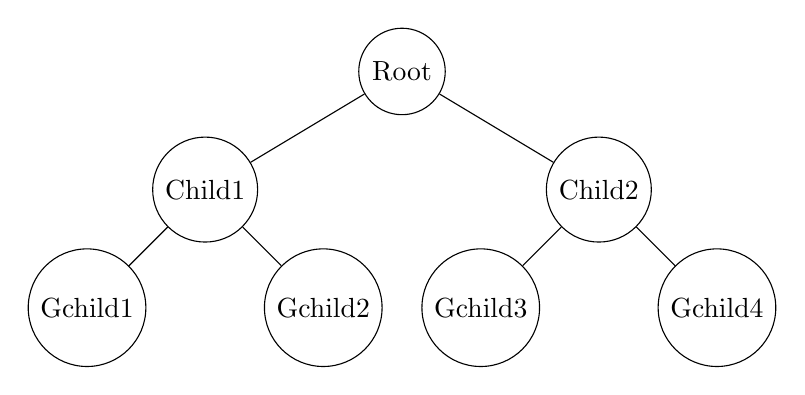
\begin{tikzpicture}[
level 1/.style={sibling distance=5cm},
level 2/.style={sibling distance=3cm},
level 3/.style={sibling distance=2cm},
every node/.style={circle,draw,align=center}
]
\node {Root}
child {node {Child1}
child {node {Gchild1}}
child {node {Gchild2}}
}
child {node {Child2}
child {node {Gchild3}}
child {node {Gchild4}}
};
\end{tikzpicture}
\caption{Hierarchy Diagram}
\label{fig:hierarchy}
\end{figure}
\end{document}